
\documentclass[11pt]{article}
\usepackage{mathtools}
\usepackage{graphicx}

\begin{document}

\begin{center}
{\bfseries \Large Scenario 1}\\
\bigskip

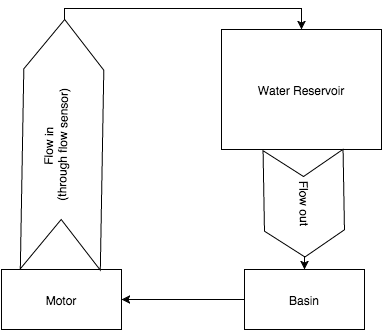
\includegraphics[scale=0.75]{Problem1}
\end{center}
\bigskip
In the first problem, we are modeling a single rig. This rig is a "leaky bucket", where water is flowing
at a constant rate out of the bucket. A PID controller then controls a motor to pump water back into the 
bucket, so that the water reaches a set height. Our challenge here is to find the volume of an object
dropped into the bucket, based on the flow rate of water into the bucket.

We will call the flow rate into the bucket, with respect to time, $f_{in}(t)$ and
the flow rate out $f_{out}$.
The volume of water added in the top chamber from $t_a$ to $t_b$ =  
$$\int_{t=t_a}^{t_b}( f_{in}(t) - f_{out} ) dt$$

If this integral has a negative value, then that volume of water was removed from the bucket in that time interval.
If an object is added into the bucket, it will displace water equal to it's volume in the bucket. Thus, the PID controller
will react and remove that volume of water from the bucket, so that the height goes back to the setpoint.
This allows for a simple way to calculate the volume of an object: The value of the above integral with $t_a$
= time that object was dropped in, and $t_b$ = time that water level steadies (or any time after). 

The flow in can be modeled in terms of the PID controller as follows:
$$e(t) = SP - h(t)$$
$$f_{in}(t) = P*(e(t)) + I*(\int_0^t e(u) du) + D*(\frac{d}{dt}e(t))$$
\bigskip
\begin{center}
{\bfseries \Large Scenario 2}\\
\bigskip
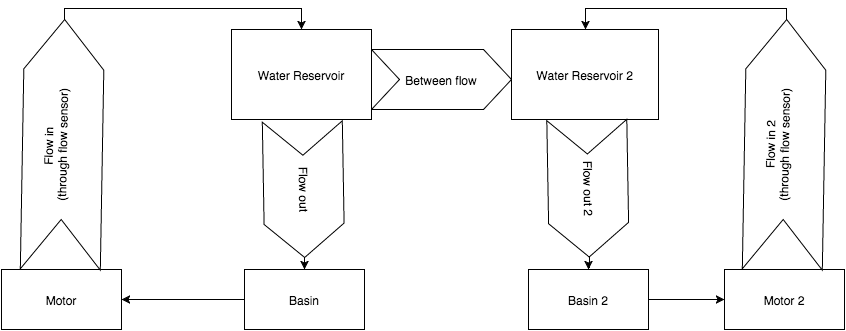
\includegraphics[scale=0.5]{Problem2}
\end{center}
\bigskip
The second scenario we are modeling is the two-bucket water height control.
This involves two connected leaky buckets, each of which needs to maintain its own setpoint.\\ \\

In order to create a mathematical model, we have to define relevant variables, and functions that define the values that those variables take over time.
In our case, we have the flow into each of the buckets $f_{in1}$ and $f_{in2}$, the flow out of each bucket (assumed to be contant) $f_{out1}$ and $f_{out2}$, the set points $SP_1$ and $SP_2$, the water heights $h_1$ and $h_2$, and the flow from bucket 1 to bucket 2 (which can be negative) $f_b$.
From these variables, we also define error variables $e_1$ and $e_2$, which are useful for simplifying the PID equations.\\ \\
Everything other than $SP_1$, $SP_2$, $f_{out1}$, and $f_{out2}$ is a function of time, and can be defined as follows for each bucket:\\
\\
$e(t) = SP - h(t)$\\ \\
$f_{in}(t) = P*(e(t)) + I*(\int_0^t e(u) du) + D*(\frac{d}{dt}e(t))$ \\ \\
$f_b(t) = (h_1(t)-h_2(t))*C$, where $C$ is determined by the size of the channel between the buckets \\ \\
$h(t) = \frac{\int_0^t (f_{in}(u)-f_{out} \pm f_b(u)) du}{D_{bucket}}$, where we subtract $f_b$ for bucket 1 and add it for bucket 2 \\ \\
In real life, and in our simulations, all of these calculations will be done in discrete time. This simplifies the equations to the following: \\ \\
$e(t) = SP - h(t)$ \\ \\
$f_{in}(t) = P*(e(t)) + I*(\sum_0^t e(t)) + D*(e(t)-e(t-1))$ \\ \\
$f_b(t) = (h_1(t)-h_2(t))*C$\\ \\
$h(t) = \frac{h(t-1)+(f_{in}(t) - f_{out}(t) \pm f_b(t))}{D_{bucket}}$\\ \\



\end{document}